\documentclass[9pt]{beamer}

\usetheme{Boadilla}

%\usepackage{extsizes}

\setbeamersize{sidebar width left=2cm}

%\setbeamercolor{palette sidebar primary}{fg=craneblue}
%\setbeamercolor{palette sidebar secondary}{fg=craneblue!75}

%\logo{
\includegraphics[height=0.8cm]{bilder/te-logo}}

\usepackage[ngerman]{babel}
\usepackage{pgf}
\usepackage{amsmath,amssymb}
\usepackage[latin1]{inputenc}
\usepackage{helvet}

\usepackage[absolute,overlay]{textpos}
\setlength{\TPHorizModule}{10mm}
\setlength{\TPVertModule}{\TPHorizModule}
\textblockorigin{0mm}{0mm}
\setlength{\parindent}{0pt}

\setbeamertemplate{sidebar canvas right}{%
	\begin{textblock}{1.5}(10.5,0.1)%
		
\includegraphics[height=0.8cm]{bilder/te-logo}%
	\end{textblock}%
	\begin{textblock}{1.5}(0.65,2.5)%
		\rotatebox{90}{\usebeamercolor[blue!60]{Sidebar}University of Erlangen-Nuremberg}%
	\end{textblock}%
	\begin{textblock}{1.5}(1.15,2)%
		\rotatebox{90}{\usebeamercolor[blue!60]{Sidebar}Institute for Electrotechnics Engineering}%
	\end{textblock}%
}
\setbeamercolor{sidebar}{bg=blue!30}

\usepackage{hyperref}
\usepackage{booktabs}
\usepackage{eurosym}

\hypersetup{
	pdftitle={Seminarvortrag, Ausarbeitung eines Praktikums zur Vorlesung ADS, LTE, Uni Erlangen-N�rnberg},
	pdfauthor={\textcopyright\ LTE Daniel Glaser},
%	pdfpagemode=FullScreen,
	pdffitwindow=true,
%	bookmarks=true,
	bookmarksopen=true,
	bookmarksopenlevel=2,
	urlcolor=green
}

\title[Ausarbeitung eines Praktikums zur Vorl. ADS]{Ausarbeitung eines Praktikums \\zur Vorlesung \\Architekturen der Digitalen Signalverarbeitung}
\author{Daniel Glaser}
\date{\today}

\subtitle{Entwurf einer Plattform und Programmierung in VHDL}

\institute[Lehrstuhl f�r Technische Elektronik]{\textbf{Lehrstuhl f�r Technische Elektronik} \\ Prof. Dr.-Ing. Dr.-Ing. habil. Robert Weigel}

\begin{document}

	\begin{frame}
	\titlepage
	
\end{frame}

\setcounter{tocdepth}{1}

\begin{frame}
  \frametitle{�bersicht}
  \tableofcontents[pausesections]
\end{frame}

\setcounter{tocdepth}{2}

\AtBeginSection[]
{
  \begin{frame}<beamer>
    \frametitle{�berblick}
    \tableofcontents[current,currentsection]
  \end{frame}
}
	
	\section{Einf�hrung}

\subsection{Motivation}

\begin{frame}
	\frametitle{Einf�hrung}
	\framesubtitle{Motivation}
	\begin{beamerboxesrounded}[shadow=true]{Vorlesung: Architekturen Digitaler Signalverarbeitung}
		\begin{itemize}[<+->]
			\item Analoge Konzepte in digitaler Hardware
			\item Algorithmen der digitalen Signalverarbeitung
			\item Optimierung von Algorithmen auf quantisierte Signale
			\item Simulationsbeispiele in MATLAB
			\item Beispiele realer Hardwareumsetzungen (Blockdiagramme)
			\item Keine Hardware "`zum Anfassen"'
			\item Fehlende praktische Erfahrung der Studenten
		\end{itemize}
	\end{beamerboxesrounded}
\end{frame}

\subsection{Zielsetzung}

\begin{frame}
	\frametitle{Zielsetzung}
	\frametitle{Entwurf eines Praktikums}
	\begin{beamerboxesrounded}[shadow=true]{Praktikum: Architekturen Digitaler Signalverarbeitung}
		\begin{itemize}
			\item<1-> Vorgabenanalyse
			\item<2-> Entwurf eines in sich geschlossenen Gesamtsytems \only<3->{$\Leftarrow$ Hagenberg}
			\item<4-> Auswahl geeigneter Konzepte aus der Vorlesung \only<5->{$\Leftarrow$ Hagenberg}
			\item<6-> Umsetzung der Algorithmen in MATLAB \only<7->{$\Leftarrow$ SA A. Schedel}
			\item<8-> Auswahl einer Hardwareplattform
			\item<9-> Entwurf eines Praktikumsskripts
			\item<10-> $\Rightarrow$ Programmierung der Algorithmen in VHDL
			\item<11-> Problemanalyse und Vorhersage
			\item<12-> Durchf�hrung des Praktikums \only<13->{$\Leftarrow$ zuk�nftig}
		\end{itemize}
	\end{beamerboxesrounded}	
\end{frame}

	
	\section{Konzept}

\begin{frame}
	\frametitle{Konzeptauswahl}
	\frametitle{Finden geeigneter Algorithmen f�r das Gesamtsytem}
	\begin{beamerboxesrounded}[shadow=true]{Gesamtsystem bestehend aus:}
		\begin{itemize}[<+->]
			\item Sender bestehend aus:
				\begin{itemize}
					\item (Pseudo-)Zufallszahlengenerator (PRN-Schieberegister)
					\item Signalgenerator (DDS, CORDIC)
					\item Modulator (FSK)
				\end{itemize}
			\item Empf�nger bestehend aus:
				\begin{itemize}
					\item Bandpassfilter (1 je Tr�gerfrequenz)
					\item H�llkurvendemodulator (1 je Tr�gerfrequenz)
					\item Tiefpassfilter (1 je Tr�gerfrequenz)
					\item Vergleicher (mit Hysterese)
				\end{itemize}
			\item Weitere Schnittstellenmodule
			\item Fehlerkorrekturhilfen
		\end{itemize}
	\end{beamerboxesrounded}
\end{frame}

\begin{frame}
	\frametitle{Konzeptdiagramme}
		\begin{center}\footnotesize
			\begin{figure}
				  \centering
						\includegraphics[width=0.8\linewidth]{bilder/FIRLinearphasenstruktur}
					\caption{FIR in Linearphasenstruktur}
			\end{figure}
		\end{center}
		\begin{center}
			\begin{figure}
				\begin{minipage}[b]{.45\linewidth}
					\centering
					  \includegraphics[width=0.9\linewidth]{bilder/prn_register}
					\caption{PRN-Register}
				\end{minipage}
				\begin{minipage}[b]{.45\linewidth}
				  \centering
						\includegraphics[width=0.7\linewidth]{bilder/sender_blockschaltbild}
					\caption{Sender Blockschaltbild}
				\end{minipage}
			\end{figure}
		\end{center}\normalsize
\end{frame}

\section{Entwickungsplattform}

\begin{frame}
	\frametitle{Entwicklungsplattform}
		\begin{beamerboxesrounded}[shadow=true]{M�glichkeiten:}
			\begin{itemize}[<+->]
				\item Rahmenbedingungen (aus Konzept)
				\item Kernkomponente FPGA
				\item Entwicklungssystem
				\begin{itemize}
					\item Verf�gbare Evaluierungsboards
					\item Design eines eigenen Systems
				\end{itemize}
			\end{itemize}
		\end{beamerboxesrounded}
		
		\only<6->{$\Rightarrow$ Eigendesign}
\end{frame}

\begin{frame}
	\frametitle{Entwicklungsplattform}
		\begin{beamerboxesrounded}[shadow=true]{Eigenes System:}
			\begin{itemize}[<+->]
				\item Rahmenbedingungen ($2 \cdot \approx 300$ \euro{}, $15 \cdot \approx 200$ \euro{})
				\item Auswahl geeigneter Bauteile
				\item Schaltplanerstellung
				\item Layout (Platzierung und Entflechtung)
				\item Aufbau
				\item Fehleranalyse
			\end{itemize}
		\end{beamerboxesrounded}
		
		\pause
		
		\begin{beamerboxesrounded}{3D-Modell des SPATES}
			\begin{center}
				\begin{figure}
					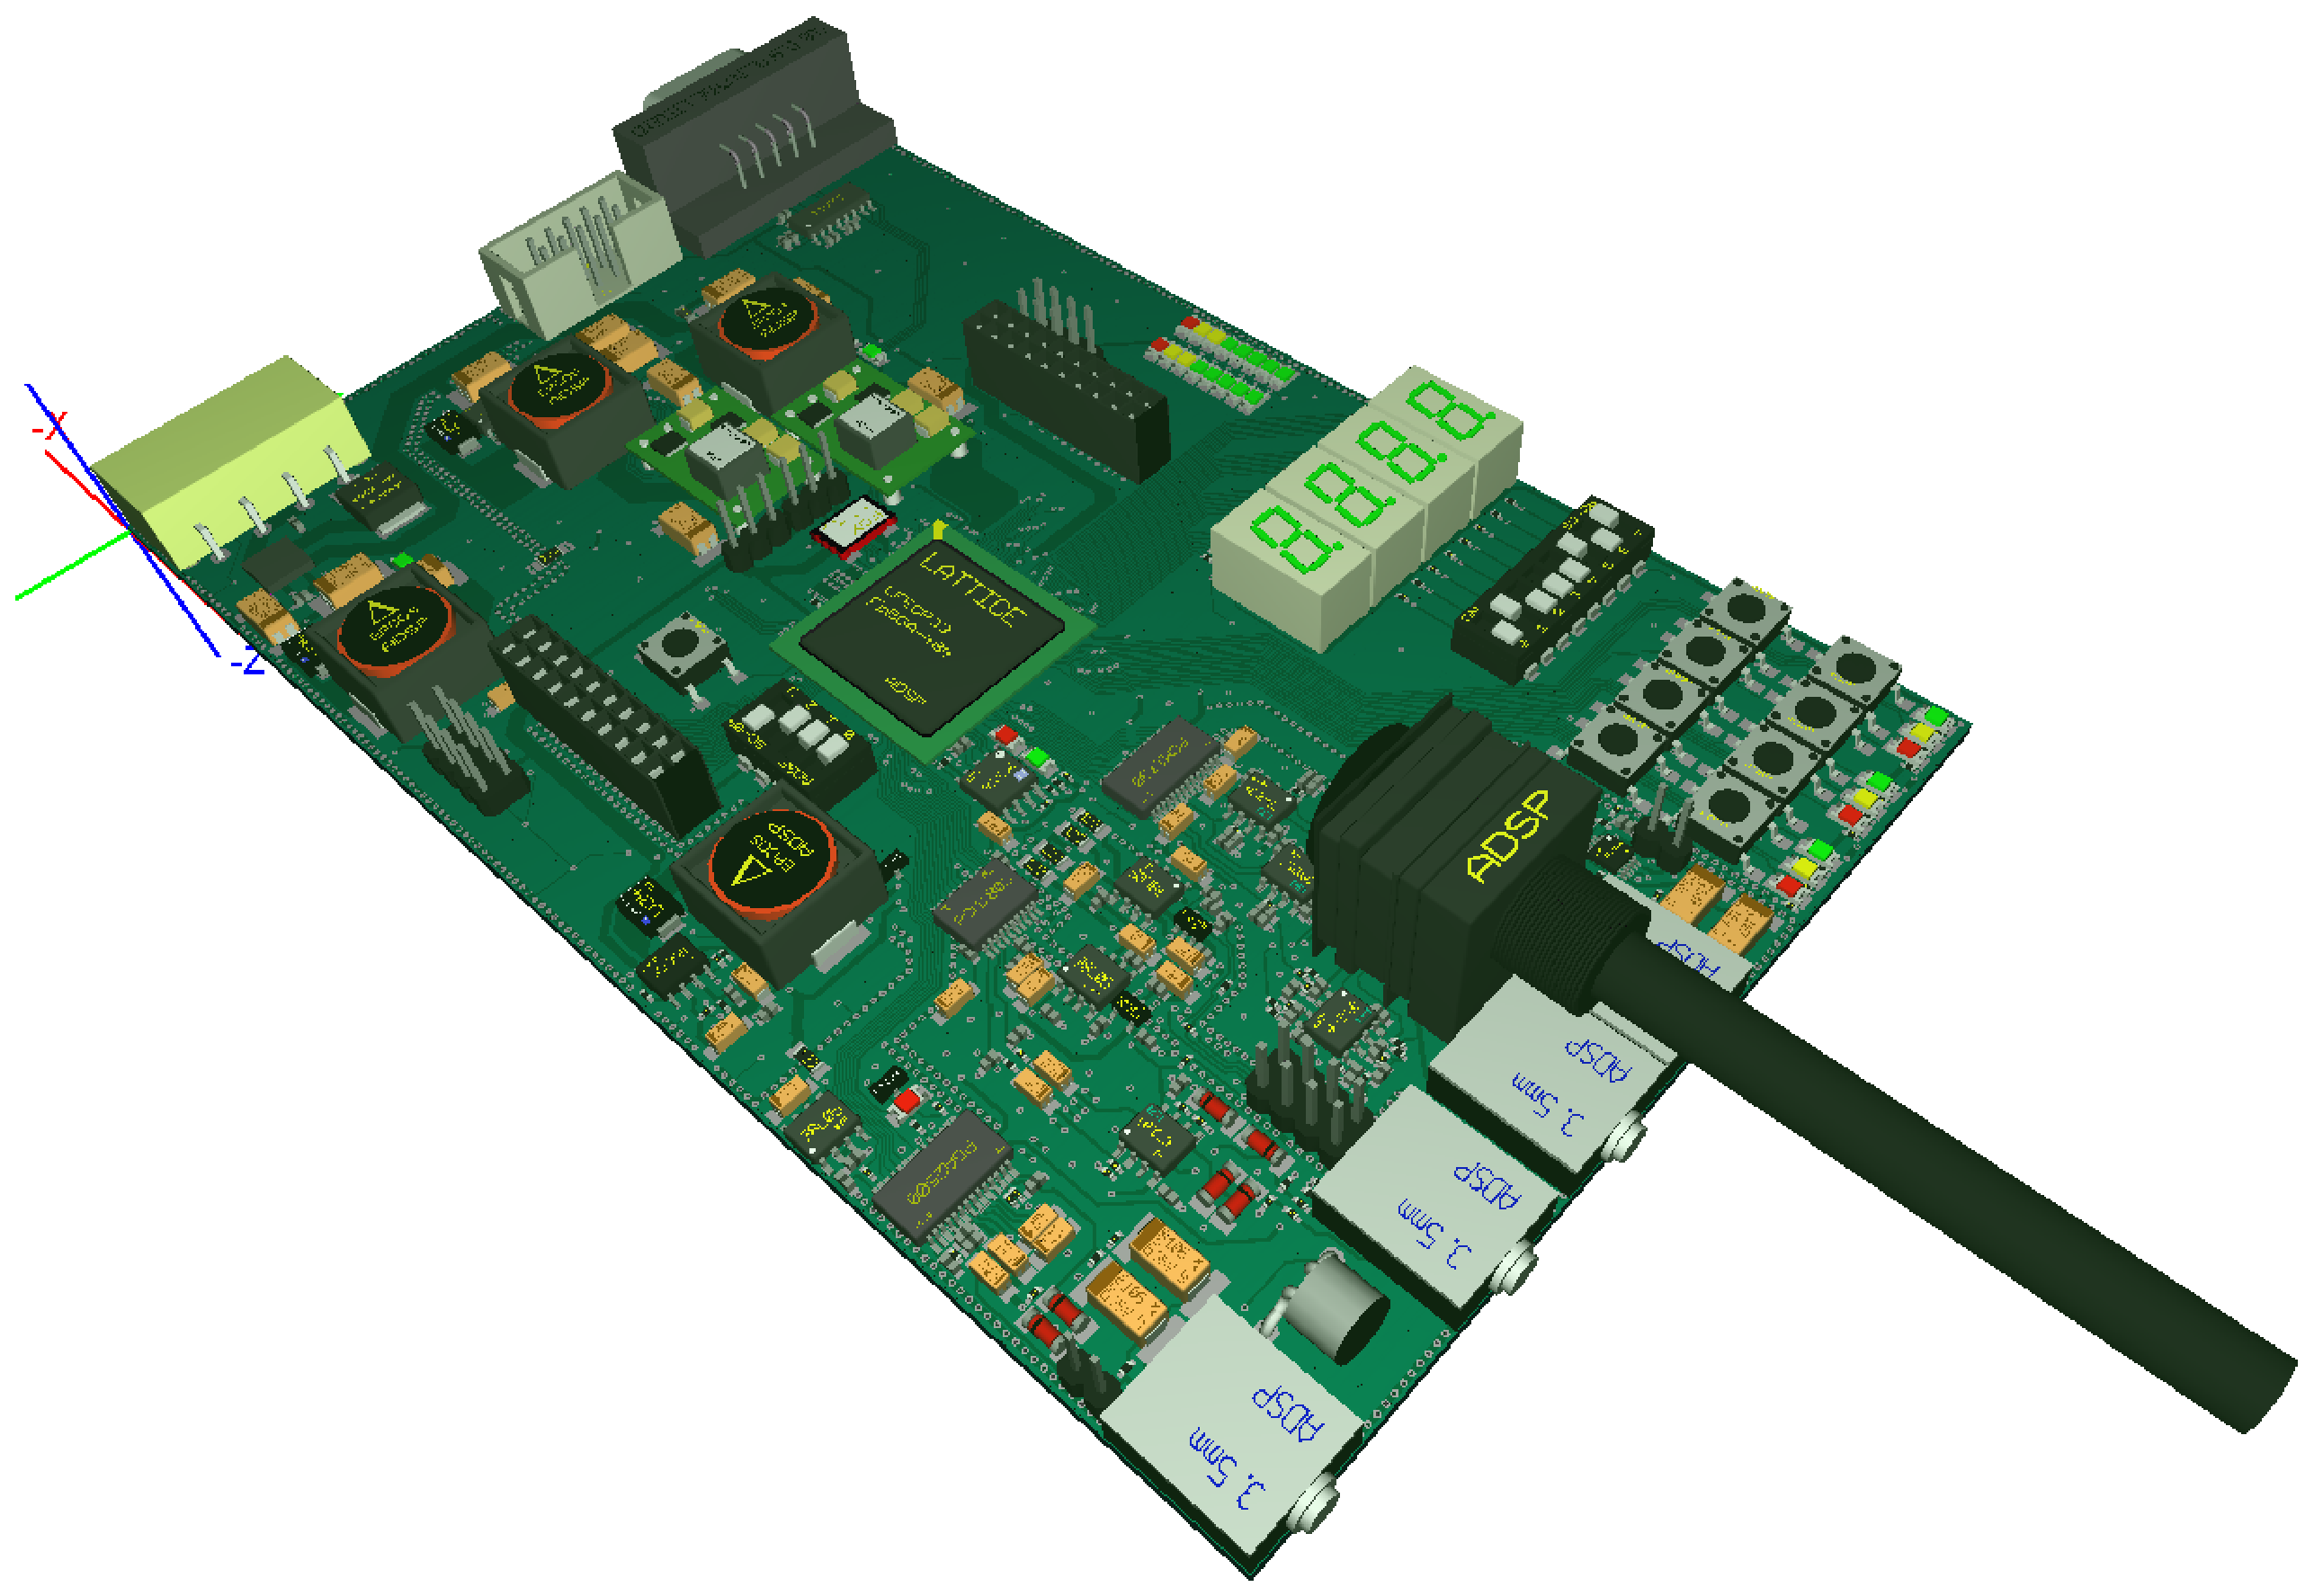
\includegraphics[width=0.6\linewidth]{bilder/ADSP-SPATES_schraeg_links_vorne}
				\end{figure}
			\end{center}
		\end{beamerboxesrounded}	

\end{frame}

\subsection{Praktikumskonzept}

\begin{frame}
	\frametitle{Praktikumskonzept}
	\framesubtitle{Abstraktion der Hardware}
	
	\begin{itemize}
		\item \alert{Grundlegend:} Starke Abstraktion der Hardware
		\item Aufbau des Wissens in kleinen Teilen
			\begin{itemize}[<+->]
				\item Vorgefertigtes Modul mit kleiner "`Leerstelle"'
				\item Grobe Vorgabe des inneren Toplevels
				\item Vorgabe der Ports
				\item V�llig selbst�ndige Programmierung der Aufgabe
			\end{itemize}
		\item Auf h�ufige Anf�nger-Fehler direkt hinweisen
	\end{itemize}
\end{frame}

\begin{frame}
	\frametitle{Abstraktionsmodell}
	\framesubtitle{Der Toplevel im Toplevel}
	\begin{beamerboxesrounded}{Hardwareabstraktion}
		\begin{center}
			\begin{figure}
				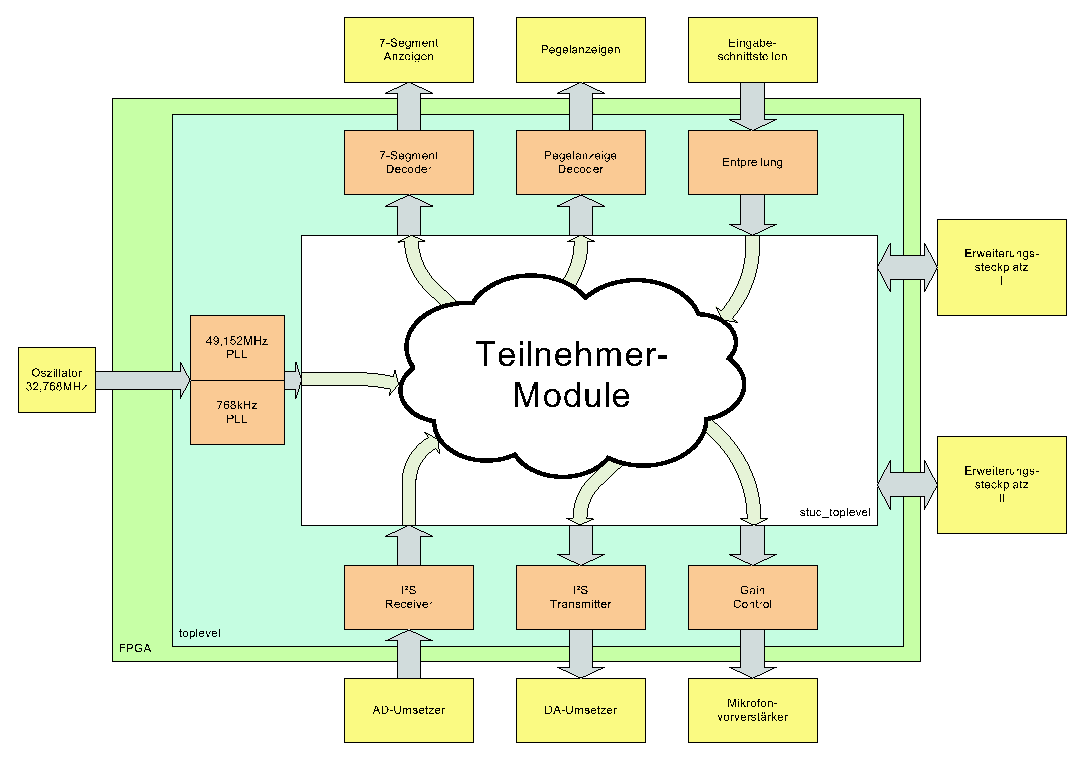
\includegraphics[width=0.8\linewidth]{bilder/hardwareabstraktion}
			\end{figure}
		\end{center}
	\end{beamerboxesrounded}	
\end{frame}
	
	\section{VHDL-Programmierung}

\subsection{Vorgefertigte Module}

\begin{frame}
	\frametitle{VHDL-Programierung}
	\framesubtitle{Hardwareabstraktion im Detail}
	\begin{beamerboxesrounded}{Vorgefertigte Module: Abstraktionmodule}
		\begin{itemize}[<+->]
			\item Initialisierungmodul
			\item Takterzeugung
			\item AD- bzw. DA-Umsetzer ($I^2S$-Schnittstelle $\Rightarrow$ parallel)
			\item Vorverst�rkerregelung
			\item 7-Segmentdecoder
			\item Mikrofonvorverst�rkerregelung
			\item Pegelanzeige-Abstraktion
			\item Schalter-/Tasterentprellung
		\end{itemize}
	\end{beamerboxesrounded}	
\end{frame}

\subsection{Musterl�sungen}

\begin{frame}
	\frametitle{VHDL-Programierung}
	\framesubtitle{Hardwareabstraktion im Detail}
	\begin{beamerboxesrounded}{Studentische Module: Musterl�sungen}
		\begin{itemize}[<+->]
			\item Erste Schritte: Multiplexer
			\item (Pseudo-)Zufallszahlengenerator
			\item Signalgenerator
			\item Pegelanzeige (f�r Fehlersuche)
			\item Modulator
			\item Bandpass (Suboptimal)
			\item Bandpass (Optimal)
			\item Demodulator
			\item Tiefpass
			\item Signalregenerierung (Hysterese)
			\item Zusammenschaltung
		\end{itemize}
	\end{beamerboxesrounded}	
\end{frame}

\subsection{Verfikation}

\begin{frame}
	\frametitle{VHDL-Programierung}
	\framesubtitle{Verifiaktion: Testbenches}
	\begin{beamerboxesrounded}{Verifikation}
		\begin{itemize}
			\item Alle Module wurden verifiziert
			\item K�nnen den Studenten als Verifikation dienen
		\end{itemize}
	\end{beamerboxesrounded}
	\begin{beamerboxesrounded}{Beispiel: Bandpass (optimal)}
		\begin{center}
			\begin{figure}
				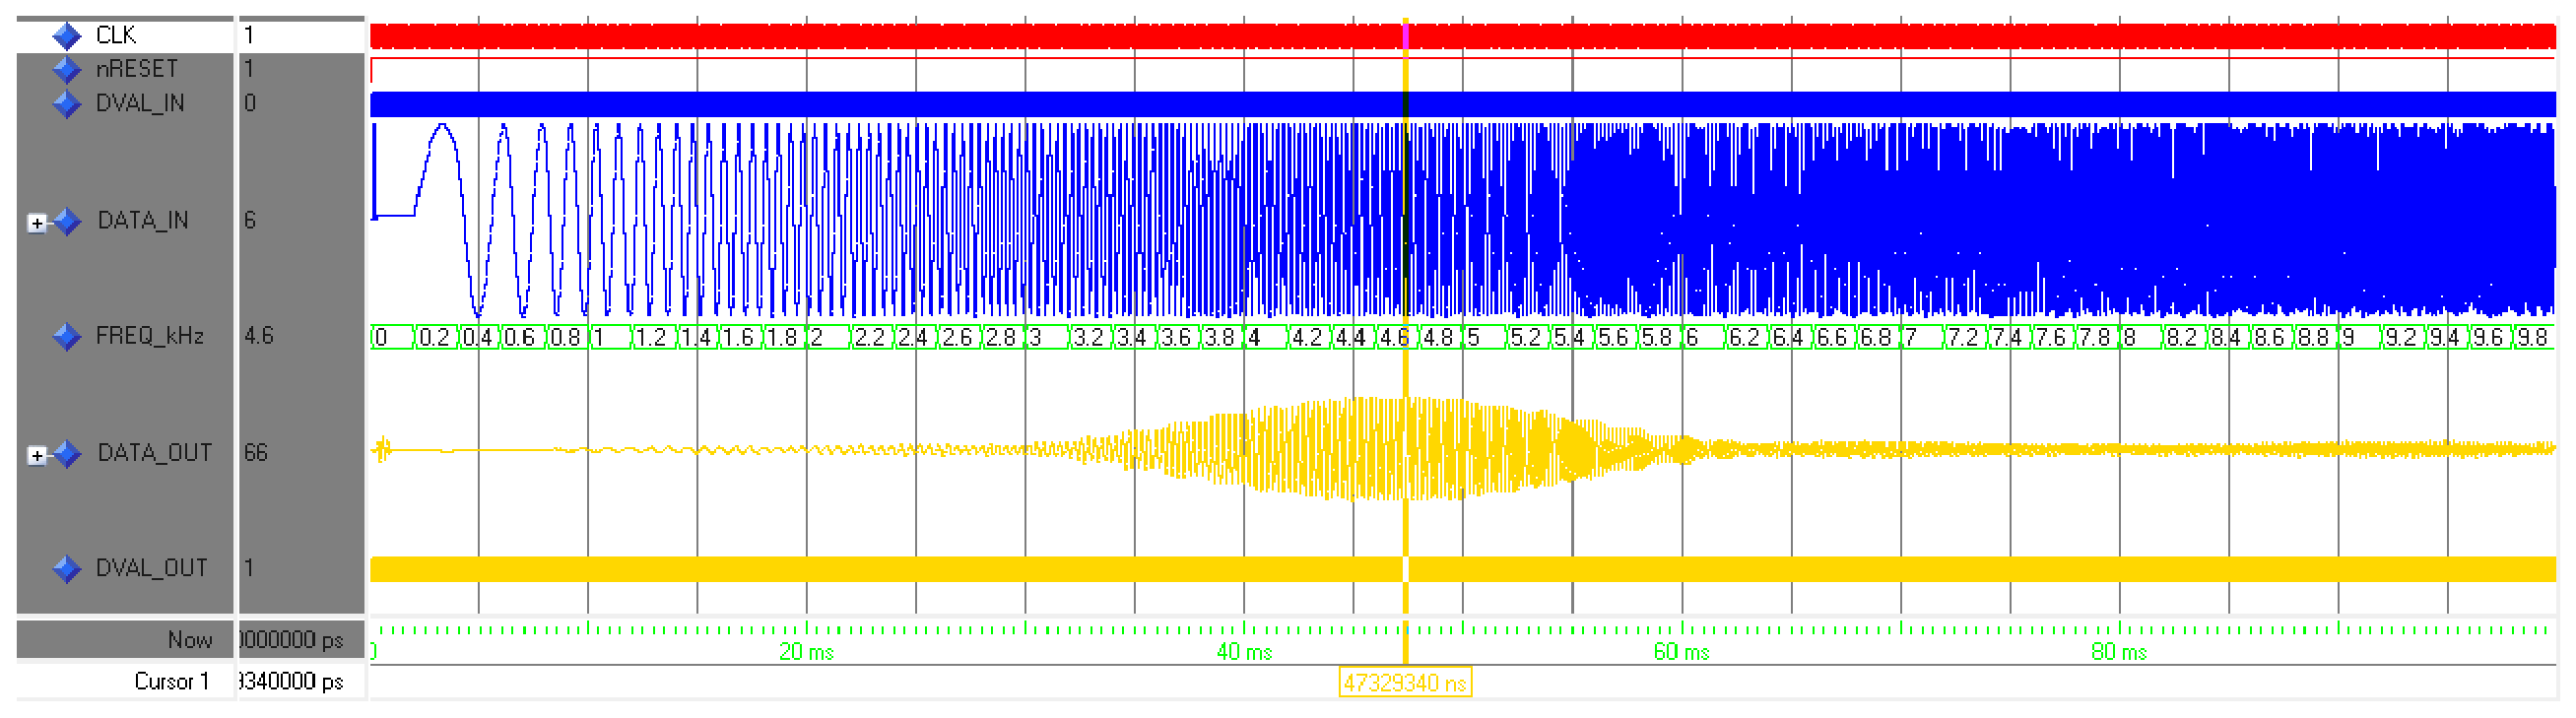
\includegraphics[width=0.8\linewidth]{bilder/filteropt}
			\end{figure}
		\end{center}
	\end{beamerboxesrounded}
\end{frame}
	
	\section{Zusammenfassung}

\subsection{Ergebnisse}

\begin{frame}
	\frametitle{Ergebnisse}
	\frametitle{Was ist fertig? Was noch zu tun?}
	\begin{beamerboxesrounded}[shadow=true]{Nacharbeit n�tig}
		\begin{itemize}[<+->]
			\item \alert{MATLAB $\Leftrightarrow$ VHDL aufeinander abgleichen}
			\item VHDL-Programierung erfolgreich
			\begin{itemize}
				\item Vorgefertigte Module arbeiten hervorragend in der Simulation
				\item Musterl�sungen sind portabel, gut strukturiert, kommentiert
				\item Testbenches auch f�r Studenten geeignet				
			\end{itemize}
			\item \alert{Hardware reparieren}
			\item VHDL-Code in Hardware verifizieren
			\item Gesamtsystem verifizieren
			\item \alert{\textbf{Den ersten Testlauf absolvieren}}
		\end{itemize}
	\end{beamerboxesrounded}	
\end{frame}

\begin{frame}
	%\frametitle{Noch Fragen?}
	\begin{beamerboxesrounded}[shadow=true]{Noch Fragen?}
		\LARGE Unklarheiten, Detailiertere Informationen?\\
		\huge Vielen Dank f�r Ihre Aufmerksamkeit!!!
	\end{beamerboxesrounded}			
\end{frame}


\end{document}